\documentclass{standalone}
  \usepackage{tikz}
  \usetikzlibrary{arrows.meta, automata, bending, positioning, shapes.misc}
  \tikzstyle{automaton}=[shorten >=1pt, >={Stealth[bend,round]}, initial text=]
  \tikzstyle{accepting}=[accepting by arrow]

\begin{document}
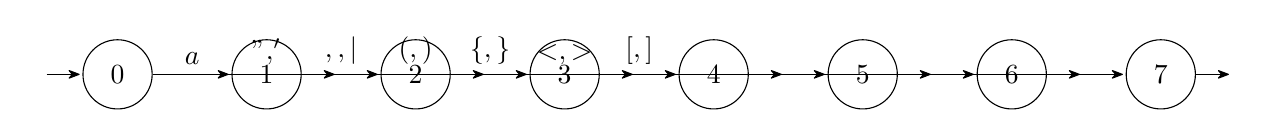
\begin{tikzpicture}[automaton, auto]
  \node[state,initial] (0) {$0$};
  \node[state,accepting] (1) [right=of 0] {$1$};
  \node[state,accepting] (2) [right=of 1] {$2$};
  \node[state,accepting] (3) [right=of 2] {$3$};
  \node[state,accepting] (4) [right=of 3] {$4$};
  \node[state,accepting] (5) [right=of 4] {$5$};
  \node[state,accepting] (6) [right=of 5] {$6$};
  \node[state,accepting] (7) [right=of 6] {$7$};
  \path[->] (0) edge node {$a$} (1);
  \path[->] (0) edge node {$", '$} (2);
  \path[->] (0) edge node {$,, |$} (3);
  \path[->] (0) edge node {$(, )$} (4);
  \path[->] (0) edge node {$\{, \}$} (5);
  \path[->] (0) edge node {$<, >$} (6);
  \path[->] (0) edge node {$[, ]$} (7);
\end{tikzpicture}
\end{document}
